%\documentclass[12pt]{article}
\input{/Users/joshyv/Research/misc/latex_paper.tex} 
\usepackage{multicol}
\usepackage{hyperref}
\newcommand{\zzz}{z}
\newcommand{\az}{\argmin_{\bM \bC \geq \ve{0}}}
\newcommand{\anx}{\argmax_{n_t \in \mathbb{N}_0 \forall t}}
\newcommand{\ann}{\argmin_{n_t \in \mathbb{N}_0 \forall t}}
\newcommand{\foopsi}{fast }

\lhead{Vogelstein JT, et al}
\rhead{Fast spike train inference from calcium imaging}
%\headheight=14.5pt

\title{Fast non-negative deconvolution for spike train inference from calcium imaging}

\author{Joshua T.~Vogelstein, Adam Packer, Tim M.~Machado, \\ Tanya Sippy, Baktash Babadi, Rafael Yuste, Liam Paninski}

\begin{document}

\maketitle
% \tableofcontents
Experiments often yield measurements of variables that are naturally constrained to be nonnegative. In such scenarios, it may be desirable to filter (or deconvolve) the observations to find the most likely trajectory of the nonnegative variable, given the noisy observations. Here, we develop a computationally-efficient optimal filter for a certain subset of nonnegatively constrained deconvolutions.  Specifically, for any nonnegative variable that is filtered by a matrix linear differential equation and observed with independent, log-concave noise, we can infer the optimal nonnegative trajectory via straightforward interior-point methods in $O(T)$ (linear) time, as opposed to more standard approaches requiring $O(T^3)$ time (where $T$ is the total number of time steps).  The key is to make use of the tridiagonal structure of the Hessian of the log-posterior here, which allows us to perform each Newton iteration in linear time.  We apply this filter to an important problem in neuroscience: inferring a spike train from noisy calcium fluorescence observations. We demonstrate the filter's improved performance on simulated and real data. In conclusion, we propose that this filter is readily applicable for a number of real-time applications, including spike inference from simultaneously-observed large neural populations.

 

\section{Introduction}

%\paragraph{Motivation}

Simultaneously imaging large populations of neurons using calcium sensors is becoming increasingly popular, both in vitro  \cite{ImagingManual} and in vivo \cite{NagayamaChen07, GobelHelmchen07, LuoSvoboda08}, especially as the signal-to-noise-ratio (SNR) of genetic sensors continues to improve \cite{GaraschukKonnerth07, MankGriesbeck08, WallaceHasan08}. Whereas the data from these experiments are movies of time-varying fluorescence signals, the desired signal is typically the spike trains or firing rates of the observable neurons.  Importantly, to a first approximation, somatic calcium concentration has a relatively simple relationship to spikes.  Thus, in theory, one could infer the most likely spike train of each neuron, given the fluorescence data.  

%\paragraph{Limitations of calcium imaging}

Unfortunately, finding the most likely spike train is a challenging computational task, for a number of reasons.  First, the signal-to-noise ratio (SNR) is often low, especially as one increases the image field and frame rate.  Second, fluorescence data typically has a low temporal resolution.  Third, to find the most likely spike train for a given fluorescence signal, one would have to search over all possible spike trains, a search that would take far too long, in practice.  

%\paragraph{Computational tools as important as experimental tools}

One is therefore effectively forced to find an approximately most likely spike train, or guess that the inferred spike train is most likely (but not really be sure).  The precise details of these approximations, however, are crucial, especially as one approaches shot-noise limited data. For in vitro studies, one often uses 1-photon imaging --- either confocal or widefield --- in which case the number of photons per neuron is a function of magnification and frame rate (obviously, other parameters, such as number of sensors per neuron, are also important, but typically more difficult to control).  To maximize the amount of information one can extract from such preparations, one should increase the frame rate and image field until achieving the shot noise limited regime, assuming one has an inference algorithm that can operate in such a scenario.  For in vivo studies, 2-photon laser scanning microscopy is currently the method of choice, for which the SNR is relatively low,  because the dwell time per pixel is (frame duration)/($\#$ of pixels in frame).  To circumvent the low SNR for in vivo studies, some groups use long integration times (e.g., \cite{OhkiReid06}), whereas others use small image fields (e.g., \cite{KerrHelmchen07}).  One would prefer to neither sacrifice temporal resolution nor number of observable neurons, to get sufficient signal quality to perform reliable inference.  Therefore, it is of the utmost importance to extract as much information as possible from the signal; especially if one is asking quantitative questions about the statistics of the spike trains from the observable neurons --- either spontaneously or in relation to some sensorimotor stimulus or other spiking neurons.

%\paragraph{Previous approaches}

A number of groups have therefore proposed algorithms to infer spike trains from calcium fluorescence data.  For instance, Greenberg et al. \cite{GreenbergKerr08} developed a novel template matching algorithm, which performed well on their data, but is not particularly computationally efficient.  Holekamp et al. \cite{HolekampHoly08} took a very different strategy, by performing the optimal linear deconvolution (i.e., the Wiener filter) on the fluorescence data.  This approach is natural from a signal processing standpoint, but does not utilize the knowledge that spikes are always positive.  In our previous work \cite{VogelsteinPaninski09}, we developed a sequential Monte Carlo method to efficiently compute the approximate probability of a spike in each image frame, given the entire fluorescence time series.   While effective, that approach is not suitable for online analyses of populations of neurons, as the computations run in approximately real-time per neuron (i.e., analyzing one minute of data requires about one minute of computational time on a standard laptop computer), and we would like real-time for a whole population of neurons.

%\paragraph{Our approach}

The present work therefore takes a somewhat different approach.  First, we carefully consider the statistics of typical data-sets, and then write down a generative model that accurately relates spiking to observations. Unfortunately, inferring the most likely spike train given this model is computationally intractable.  We therefore make some well-justified approximations, which lead to an algorithm that infers the approximately most likely spike train, given the fluorescence data.  Our algorithm has a few particularly noteworthy features, relative to other approaches.  First, we assume that spikes are always positive.  This assumption often improves filtering results when the underlying signal has this property \cite{LeeSeung99, LeeSeung01, HuysPaninski06}.  Second, our algorithm is extremely fast: it can process a calcium trace from 50,000 images in about one second on a standard laptop computer. In fact, filtering the signals for an entire population of about $100$ neurons runs \emph{faster} than real time. This speed facilitates using this filter online, as observations are being collected. In addition to these two features, we can generalize our model in a number of ways, including incorporating spatial filtering of the raw movie. The efficacy of the proposed filter is demonstrated on several real data-sets, suggesting this algorithm is a powerful and robust tool for online spike train inference.  The code (which is a simple Matlab script) is available from the authors upon request. 

As described above, to develop an algorithm to approximate the most likely spike train given fluorescence data, we first carefully analyze the statistics of typical data-sets.  We start by considering an in vitro experiment, for which the SNR is relatively high, and build an appropriate generative model (Section \ref{sec:model}).  Given this model, we can formally state our goal (Section \ref{sec:goal}).  And given this goal, we derive an approximately optimal inference algorithm (Section \ref{sec:inf}).  We then generalize our model in a number of ways, incorporating spatial filters (Section \ref{sec:spatial}), overlapping spatial filters (Section \ref{sec:overlap}), Poisson observations (Section \ref{sec:poisson}), fluorescence saturation (Section \ref{sec:satur}), and slow rise time for genetic sensors (Section \ref{sec:slow}).  Inferring the most likely spike train in all the above scenarios requires having an estimate of the parameters governing the relationship between the spikes and the movie.  Thus, we also develop an approach to efficiently approximate the maximum likelihood estimate (MLE) of the parameters (Section \ref{sec:learn}).  Finally, we describe several measures we use to assess and compare performance of our algorithm with others (Section \ref{sec:ass}).    

\section{Results} \label{sec:results}

\subsection{Main Result} \label{sec:main}

The main result of this paper is that we can approximate $\hbn$ very efficiently, and that this approach outperforms a more \naive approach of a typical deconvolution filter, half-wave rectified (i.e., setting everything below zero equal to zero).  Fig. \ref{fig:woopsi_inf} depicts a simulation showing this result. Clearly, the \foopsi filter is outperforming the optimal linear deconvolution filter (also called a Wiener filter).  The Wiener filter implicitly approximates the Poisson spike rate with a Gaussian spike rate (see Appendix for details). While a Gaussian well approximates a Poisson distribution when rates are about $10$ spikes per frame, this example is obviously very far from that regime, and so the Gaussian approximation does very poorly. Furthermore, the Gaussian approximation allows for the inferred spike train to include negative numbers, which we do not want, as spike trains are non-negative entities.  To counteract the negative values, the Wiener filter then infers large positive values, contributing to a ``ringing'' effect.  The non-negative constraint imposed by the \foopsi filter ensures that such ringing does not take place.  Finally, by utilizing Gaussian elimination and interior-point methods, as described in the Methods section, the computational complexity of \foopsi filter is the same as an efficient implementation of the Wiener filter.  


\begin{figure}[h!]
\centering 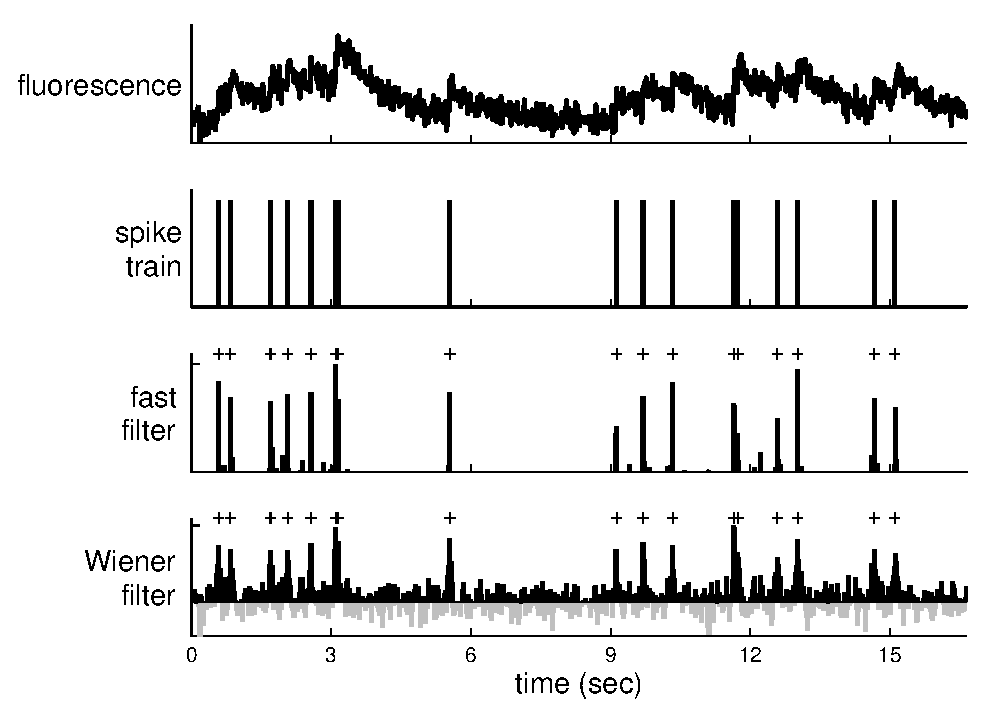
\includegraphics[width=.9\linewidth]{../figs/woopsi_inf}
\caption{The \foopsi filter significantly outperforms the optimal linear deconvolution (aka, Wiener) filter on typical simulated data-sets. Top panel: fluorescence trace.  Second panel: spike train.  Third panel: \foopsi filter inference.  Bottom panel: Wiener filter inference.  Gray '$+$'s in bottom two panels indicate true spike times.  Simulation details: $T=2930$ time steps, $\Del=5$ msec, $\alpha=1$, $\beta=0$, $\sig=0.3$, $\tau=1$ sec, $\lam=1$ Hz.} \label{fig:woopsi_inf}
\end{figure}


In the above, we assumed that we knew the model parameters of interest.  However, in the general case, the parameters are unknown, and must therefore be estimated from the data.  In Section \ref{sec:learn} we described how the parameters of our model may be estimated directly from the observations.  Importantly, this obviates the need to conduct joint imaging and electrophyiological experiments to obtain ``training'' data, as the developed approach is fully unsupervised.  Figure \ref{fig:woopsi_learn} shows another simulated example; in this example, however, the parameters are estimated from the observed fluorescence trace.  Again, it is clear that the \foopsi filter far outperforms the Wiener filter.

\begin{figure}[h!]
\centering 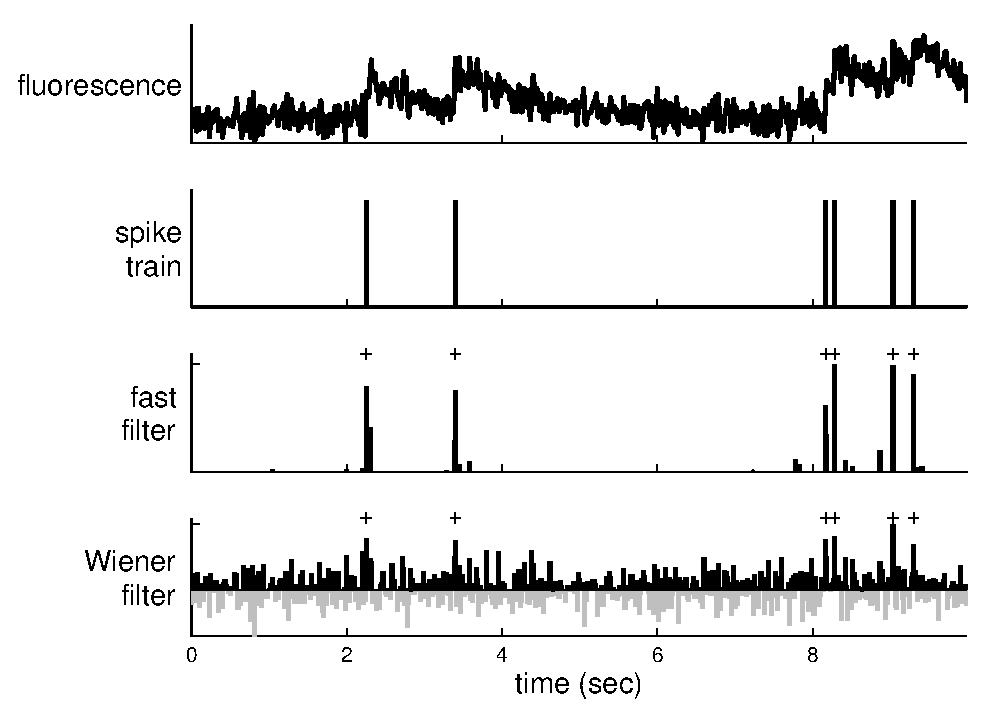
\includegraphics[width=.9\linewidth]{../figs/woopsi_learn}
\caption{The \foopsi filter significantly outperforms the Wiener filter, even when estimating the parameters only from the observed data.  Simulated details as in Figure \ref{fig:woopsi_inf}.} \label{fig:woopsi_learn}
\end{figure}

Given the above two results, we then applied this \foopsi filter to real data.  More specifically, by simultaneously recording electrophysiologically and imaging, we can determine the true spike times, and then compare the accuracy of the two filters.  Figure \ref{fig:woopsi_data} shows similar result for this typical in vitro data-set.  These results are typical of the 12 joint electrophysiological and imaging experiments conducted (not shown). Note that the first few ``events'' are actually pairs of spikes, which is reflected in the inferred spike trains.

\begin{figure}[h!]
\centering 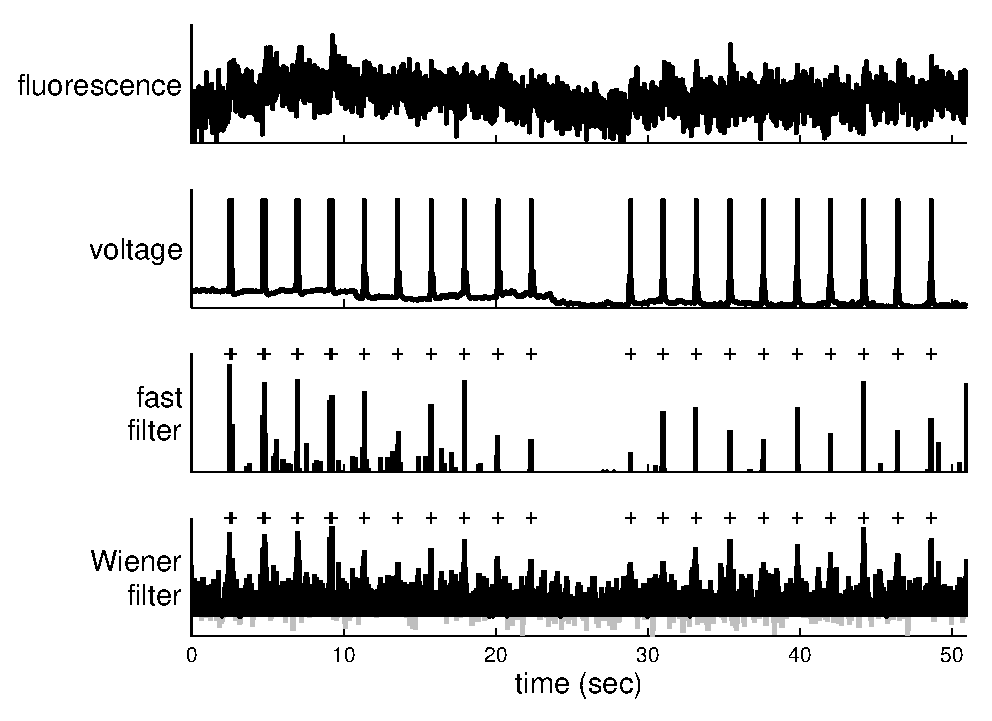
\includegraphics[width=.9\linewidth]{../figs/woopsi_data4}
\caption{The \foopsi filter significantly outperforms the Wiener filter on typical in vitro data-sets.  Note that all the parameters for both filters were estimated from the data.} \label{fig:woopsi_data}
\end{figure}

\subsection{Online analysis of spike trains using the \foopsi filter}

A central aim for this work was the development of a algorithm that infers spikes sufficiently efficiently to use online while imaging a large population (eg, $\approx 100$) of neurons.  Figure \ref{fig:pop} shows the result of running \foopsi on 136 neurons, recorded simultaneously, as described in the Methods section.  Note that the filtered fluorescence signals much more clearly show fluctuations in spiking. These spike trains were inferred in approximately real time, meaning that one could infer spike trains for the past experiment while conducting the subsequent experiment.


\begin{figure}[h!]
\centering 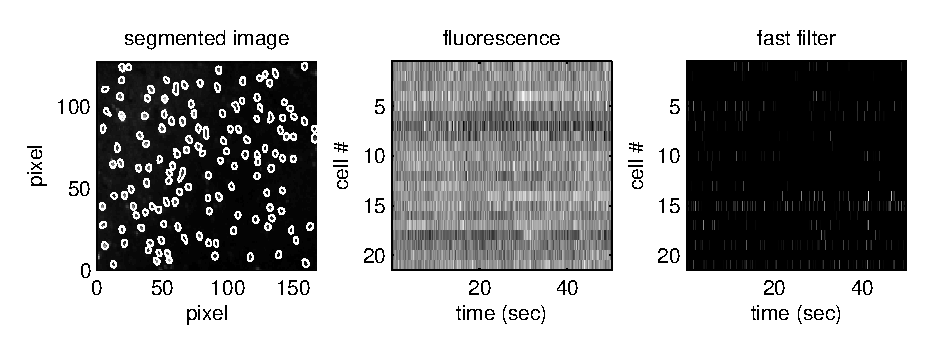
\includegraphics[width=.9\linewidth]{../figs/pop}
\caption{Applying the \foopsi filter in real time to a large population of neurons imaged simultaneously.  The inferred spike trains convey much more clearly the neural activity.  Left panel: Mean segmented image field.  Middle panel: example fluorescence traces.  Right panel: \foopsi filter output corresponding to each associated trace.} \label{fig:pop}
\end{figure}


\subsection{Improving inference results}

In Section \ref{sec:model}, we described a simple principled first-order model relating the spike trains to the fluorescence trace.  A number of the simplifying assumptions that we made above can be straightforwardly relaxed.  We tried relaxing three in particular: the linearity between calcium and fluorescence, the Gaussianity of the noise on the fluorescence measurements, and the static nature of the prior, $\lam$.  Combining all three of these modifications yields a more powerful model:


\begin{align}
	F_t &\sim \text{Poisson}(\alpha S(C_t) + \beta) \label{eq:nonlin} \\
	% C_t &= (1-\Del/\tau)C_{t-1} + n_t
	n_t &\sim \text{Poisson}(\lam_t \Del),
\end{align}

\noindent where the dynamics for calcium are as before, and we take $S(C_t)=\frac{C_t}{C_t + k_d}$ to be the standard Hill equation \cite{PologrutoSvoboda04}.  To modify our \foopsi filter to be optimal for this new model, we must simply compute the gradient and Hessian for the MAP estimate of this new model.  Note that both the Poisson observation assumption and the time-varying assumption maintain the log-concavity of the posterior, meaning that by using Newton-Raphson, we are still guaranteed to converge to the globally optimal solution.   

Unfortunately, using this more powerful model did not result in substantial inference improvements for simulated or in vitro data (not shown).  This is possibly due to approximating the Poisson distribution governing spiking with an exponential distribution.  This approximation is required to ensure concavity of the posterior.  In previous work, we developed a sequential Monte Carlo (SMC) method to infer spike trains \cite{VogelsteinPaninski09}, that does not require such an assumption. Like the fast filter, the SMC filter estimates the model parameters in a completely unsupervised fashion, ie, from the fluorescence observations, using an expectation-maximization algorithm.  Previously, we initialized parameters for the SMC filter based on other data-sets.  While effective, this initialization was often far from the final estimates, and therefore, required a relatively large number of iterations (eg, 20-25) before converging.  Thus, we reasoned that we could use the \foopsi filter to improve the initial parameter estimates, and reduce the required number of iterations.  Indeed, Figure \ref{fig:smc_init} shows how the SMC filter outperforms the \foopsi filter on in vitro data, and only required $3$--$5$ iterations to converge.  Note that the first few events are individual spikes, resulting in relatively small fluorescence fluctuations, whereas the next events are actually spike doublets, causing a much larger fluorescence fluctuation.  Only the SMC filter picks up the individual spikes in this trace, a result typical when the effective signal-to-noise ratio (SNR) is so poor.  Thus, these two inference algorithms are complementary: the \foopsi filter can be used for rapid, online inference, and for initializing the SMC filter, which can then be used to further refine the spike train estimate.

\begin{figure}[h!]
\centering 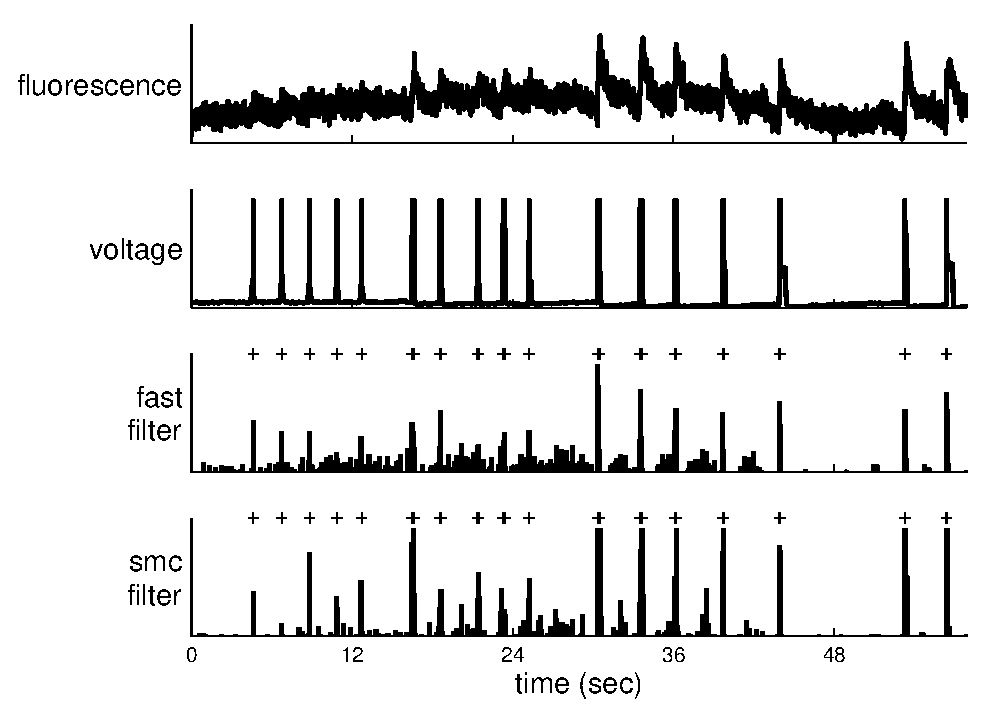
\includegraphics[width=.9\linewidth]{../figs/smc_init12}
\caption{The \foopsi filter effectively initializes the parameters for the SMC filter (which outperforms the \foopsi filter), significantly reducing the number of expectation-maximization iterations to convergence.  Note that the ordinate on the bottom panel corresponds to the probability of a spike having occurred in each frame.} \label{fig:smc_init}
\end{figure}

\subsection{Spatial filter}

In the above, we assumed that the data was a one-dimensional fluorescence trace.  In actuality, the data is a time series of images, which are first segmented into regions-of-interest (ROI), and typically, then averaged, to obtain $F_t$.  In theory, one could improve the effective SNR of the fluorescence trace by scaling each pixel relative to one another.  In particular, pixels not containing any information about calcium fluctuations can be ignored, and pixels that are approximately anti-correlated with one another could have weights with opposing signs.  

Figure \ref{fig:spatial} demonstrates the potential utility of this approach.  The top row shows different depictions of an ROI containing a single neuron.  On the far left panel is the true spatial filter for this neuron.  This particular spatial filter was chosen based on our experience analyzing both in vitro and in vivo movies; often, it seems that the pixels immediately around the soma are anti-correlated with those in the soma.  This effect is possibly due to the influx of calcium from extracellular space immediately around the soma.  This simulated movie is relatively noisy, as indicated by the second panel, which depicts an exemplary image frame.  The standard approach, given such a noisy movie, would be to first segment the movie to find an ROI corresponding to the soma of this cell, and then spatially average all the pixels found to be within this ROI.  The third panel shows this ``typical spatial filter''.  The forth panel shows the mean frame, ie, $\langle \vbF \rangle_t$.  Clearly, this mean frame is very similar to the true spatial filter.

The bottom panels of Figure \ref{fig:spatial} depict the effect of using the true spatial filter, versus the typical one. The left side shows the fluorescence trace and its associated spike inference obtained from using the typical spatial filter.  The right side shows the same when using the true spatial filter.  Clearly, the true spatial filter results in a much cleaner fluorescence trace and spike inference.  


\begin{figure}[h!]
\centering 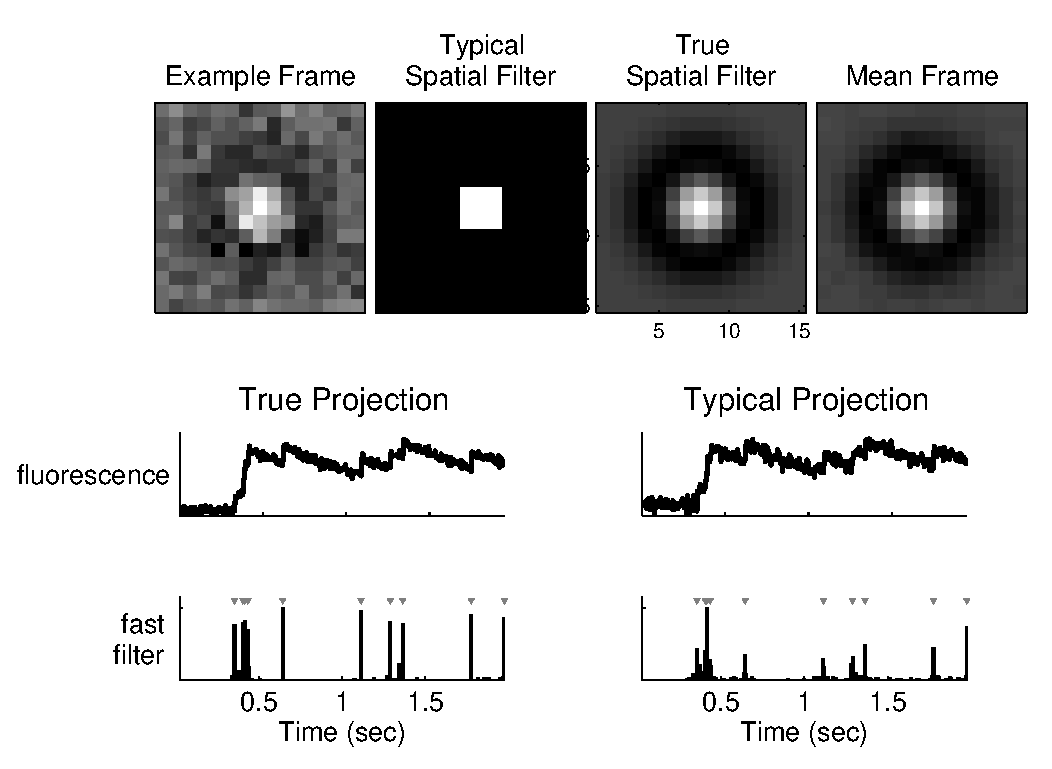
\includegraphics[width=.9\linewidth]{../figs/spatial2}
\caption{A simulation demonstrating that using a better spatial filter can significantly enhance the effective SNR (see Supplementary Movie 1 for the full movie associated with this simulation). We modeled the true spatial filter as a sum of Gaussians: a positively weighted small variance Gaussian, and a negatively weighted large variance Gaussian (both with the same mean).  Top row far left: true spatial filter.  Top row second from left: example frame (frame number 100). Top row second from right: typical spatial filter.   Top row far right: mean frame.  Middle row left: fluorescence trace using typical spatial filter. Bottom row left: \foopsi filter output using typical spatial filter.  Middle row right: fluorescence trace using true spatial filter.  Bottom right: \foopsi filter output using true spatial filter. Simulation details: $\valpha=\mN(\ve{0},2 \bI)-1.1 \mN(\ve{0},2.5 \bI)$ where $\mN(\ve{mu},\ve{\Sig})$ indicates a Gaussian with mean $\ve{\mu}$ and covariance matrix $\ve{\Sig}$, $\bbeta=1$, $\tau=0.85$ sec, $\lam=5$ Hz.} \label{fig:spatial} 
\end{figure}



\subsection{Overlapping spatial filters}


The above shows that if a ROI contains only a single neuron, we can enhance the effective SNR by spatially filtering.  However, this analysis assumes that only a single neuron is in the ROI.  Often, neural spatial filters are overlapping, or nearly overlapping, making the segmentation problem even more difficult.  Therefore, it is desirable to have an ability to crudely segment, yielding only a few neurons in each ROI, and then spatially filtering within each ROI to pick out the spike trains from each neuron.  We can do this in a principled manner by generalizing our model as described in Section \ref{sec:methods:overlapping}.  Figure \ref{fig:spatial_multi_inf} shows an example of this approach on simulated data. Note that the spatial filters are sufficiently overlapping that some ``bleed-though'' can be seen across the traces.  


\begin{figure}[h!]
\centering 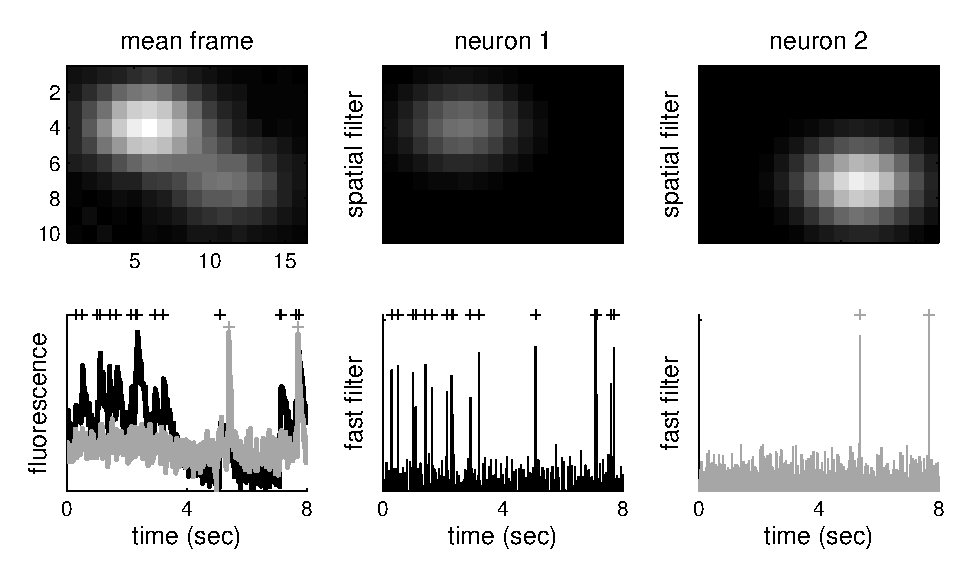
\includegraphics[width=.9\linewidth]{../figs/spatial_multi_inf}
\caption{Simulation showing that even when two neurons' spatial filters are overlapping, one can separate the two signals by spatial filtering. Simulation details: $\valpha^1=\mN([-1.8 1.8],2 \bI)\, \valpha^2=\mN([1.8 -1.8],5 \bI)$, $\bbeta=[1 1]\T$, $\tau=[0.5 0.5]\T$ sec, $\lam=[1.5 1.5]$ Hz.} \label{fig:spatial_multi_inf}
\end{figure}

While Figure \ref{fig:spatial_multi_inf} shows that one could separate the signals if the spatial filters of the neurons were known, FIgure \ref{fig:spatial_multi_learn} shows that we can estimate the spatial filters, using only the fluorescence movie, using the approach described in Section \ref{sec:methods:overlapping}.


\begin{figure}[h!]
\centering 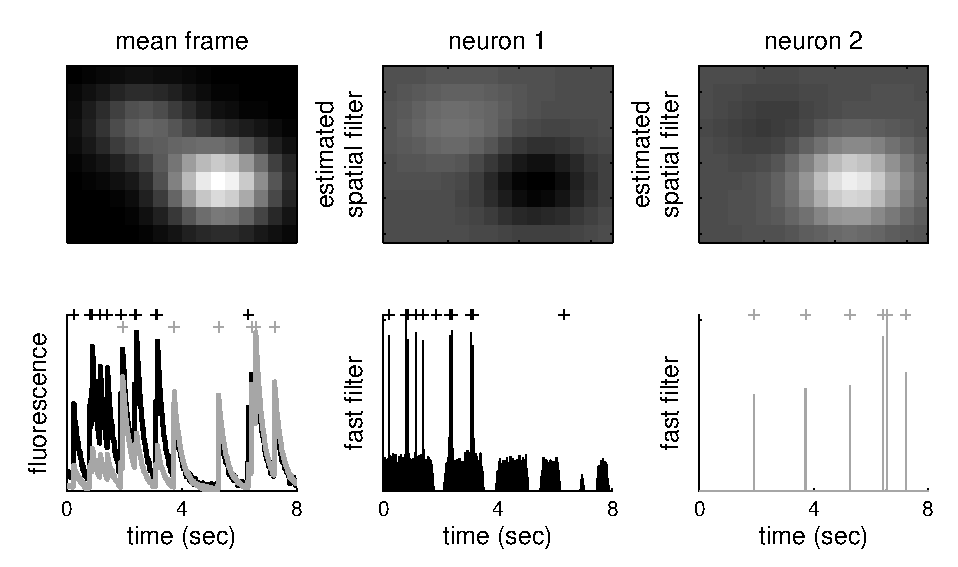
\includegraphics[width=.9\linewidth]{../figs/spatial_multi_learn}
\caption{Simulation showing that even when two neuron's spatial filters are largely overlapping, we can infer the spatial filter of each, to separate the two signals. Simulation details as above.} \label{fig:spatial_multi_learn}
\end{figure}



We show here that for certain nonnegative deconvolution problems, we can derive an algorithm that is both optimal and efficient.  More specifically, our algorithm may be applied to any model with a nonnegative signal that is linearly filtered by a matrix linear ordinary differential equation.  We apply this approach to the problem of inferring the most likely spike train given noisy calcium sensitive fluorescence observations (c.f. Fig.\ \ref{fig:demo}), and demonstrate, in simulations, that the optimal nonnegative filter outperforms the optimal linear (i.e., Wiener) filter in both slow and fast firing rate regimes (c.f. Fig.\ \ref{fig:comp}).  Furthermore, when applied to data from a live cell, the optimal nonnegative filter outperforms a fast projection pursuit regression filter, which constrains the inferred spike train to be nonnegative integers (c.f. Fig.\ \ref{fig:real}). On the other hand, the nonnegative filter is based on a linear observation model, and therefore suffers a loss of precision in the presence of strong saturation effects, in contrast to the optimal nonlinear particle filter (c.f. Fig.\ \ref{fig:real}).    

The implications of these results are severalfold.  First, it seems as if there is no reason to use the Wiener filter for scenarios in which our algorithm may apply.  Second, as our filter is so efficient, it may be used for many real-time processing applications.  Specifically, upon simultaneously imaging a population of neurons \cite{IkegayaYuste04, NiellSmith05, OhkiReid05, YaksiFriedrich06, SatoSvoboda07}, our filter may be applied essentially online.  This could greatly expedite the tuning of important experimental parameters --- such as laser intensity --- to optimize signal-to-noise ratio for inferring spikes.  Third, the parameters estimated from this filter may be used to initialize the parameters of the optimal nonlinear particle filter, which may then be used offline, to further refine the spike train inference. % Because the optimal nonlinear particle filter performs in approximately real-time (making it $\sim 100$ fold slower than the filters developed here), it may be run overnight on all the neural data collected in a daily experimental session. 
%Future work will consider multidimensional models for this application, incorporating both more sophisticated calcium models, and spatial filtering for extracting the fluorescence signal, obviating the need for additional algorithms for image segmentation. 



\paragraph{Acknowledgments}

The authors would like to express appreciation for helpful discussions with Vincent Bonin.  Support for JTV was provided by NIDCD DC00109. LP is supported by an NSF CAREER award, by an Alfred P.\ Sloan Research Fellowship, and the McKnight Scholar Award. RY's laboratory is supported by .  LP and RY share .

%\subparagraph*{References}
\bibliography{/Users/joshyv/Research/misc/biblist}
\addcontentsline{toc}{section}{References}
%\bibliography{Science}
%\bibliographystyle{apalike}
\bibliographystyle{unsrt}
%\bibliographystyle{nature}


\appendix
When the observed neuron is spiking quickly, the Poisson distribution may be well approximated by a Gaussian distribution, suggesting that the Wiener filter may be optimal in this regime.  But the exponential approximation of a Poisson is also very accurate in the fast spiking regime.  To compare these two strategies, we simulated a fast spiking neuron, where the expected number of spikes per bin exceeds 10 (Fig. \ref{fig:FastSpiking}). In this scenario, both the Wiener filter and our fast filter perform approximately equally well.  Both filters infer peaks in the firing rate that are obscured by the low-pass filter properties of the calcium dynamics. Thus, it seems from this analysis that regardless of the firing rate of the observable neuron, (1) filtering the signal may provide valuable information, and (2) our fast filter performs at least as well as the Wiener filter, without requiring more computational time.


\newpage \begin{figure}[H]
\centering 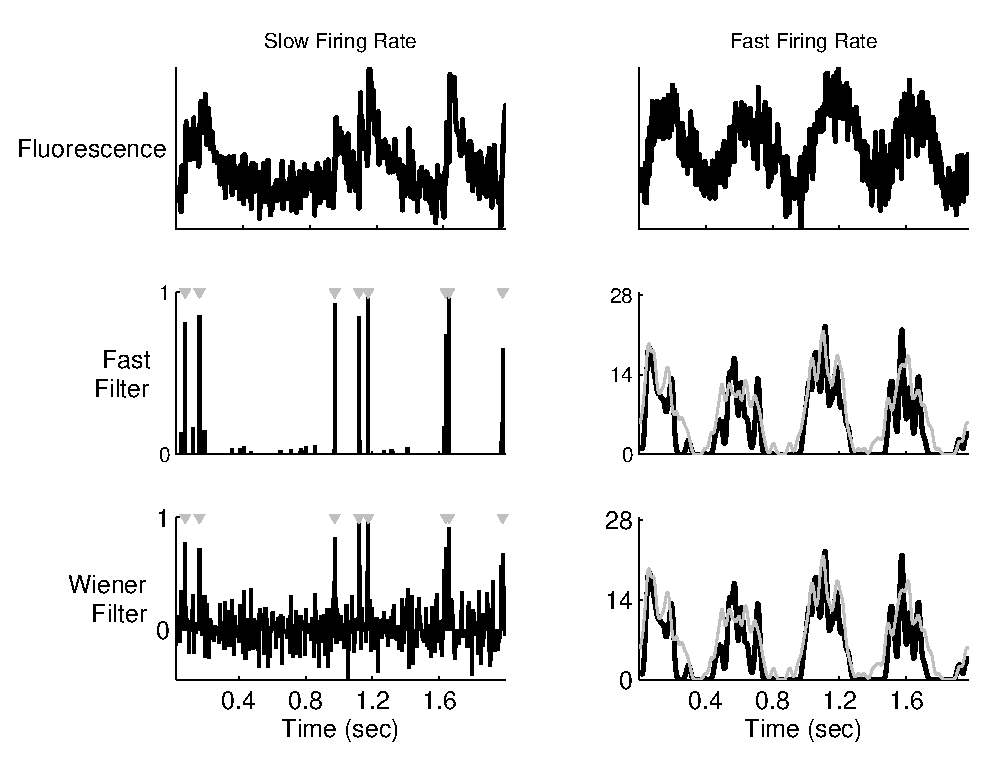
\includegraphics[width=.9\linewidth]{../figs/wiener}
\caption{A simulation demonstrating that the fast filter performs at least as well as the optimal linear filter. The left panels show that in the slow firing  regime, the fast filter --- which approximates the Poisson distribution governing spiking with an exponential distribution  --- outperforms the Wiener filter --- which approximates the Poisson distribution with a Gaussian.  The right panels show that both approximations are sufficient in the fast firing regime. Top left panel: fluorescence time series for a neuron with a slow firing rate.  Middle left panel: the fast filter's inferred spike train.  Bottom left panel: Wiener filter's inferred spike train.  Note that (i) the Wiener filter does not impose a non-negativity constraint, and (ii) the effective SNR of this filter in this example is higher than the fast filter's.  Top right panel: same as top left panel, for a neuron with a high firing rate.  Middle right panel: the fast filter's inferred spike train smoothed with a Gaussian kernel for visualization purposes (black line), and the true spike train smoothed with the same Gaussian kernel (gray line).  Bottom right panel: same as middle right panel, but with the Wiener filter. Parameters for left panels: same as above.  Parameters for right panels: same as above, except: $\sig=8$ a.u., $\lam=500$ Hz.} \label{fig:wiener}
\end{figure}

\newpage \begin{figure}[H]
%\centering 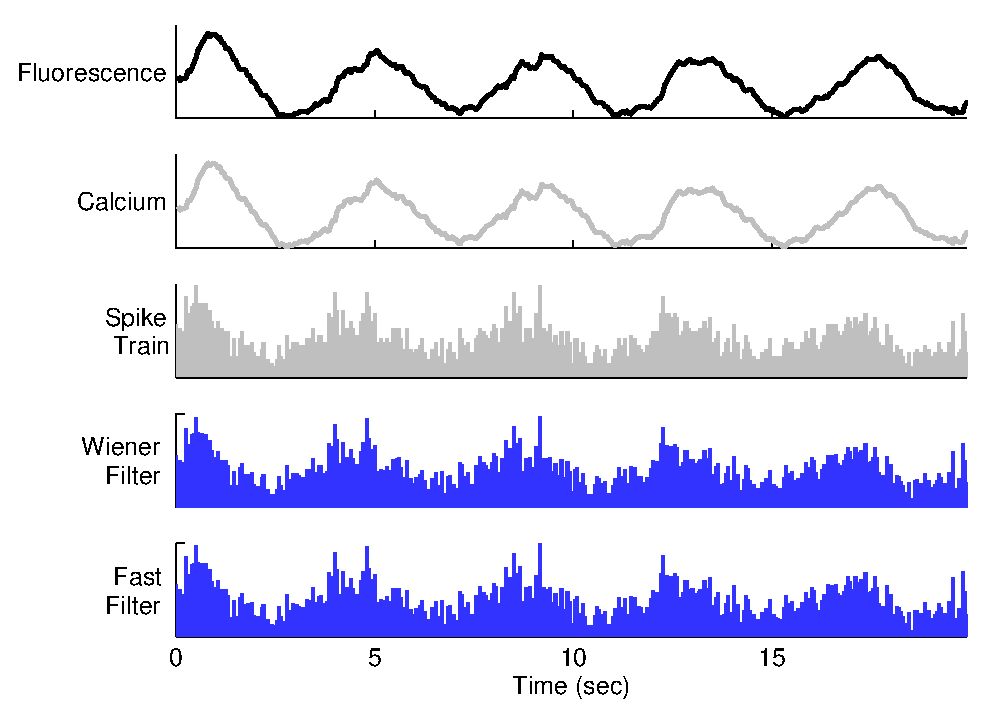
\includegraphics[width=.9\linewidth]{FastSpiking}
\caption{Comparing the Wiener filter and our fast filter for a fast spiking neuron.  In this scenario, the two filters perform approximately equally well. Note that both recover fast fluctuations in the firing rate that are smoothed out by the calcium dynamics. Conventions as in Fig. \ref{fig:schem}.  Actual and inferred spike trains were normalized similarly, to ease comparisons. Parameters: $\gamma=0.94$, $\nu=0$, $\rho=1$, $\sig=0.3$, $\lam=100$ (modulated by a sinusoid), $\Del=0.05$ msec.} \label{fig:FastSpiking}
\end{figure}




% \subsubsection{Poisson observations}
\paragraph{Model}

\begin{align}
	F_t \sim \text{Poisson}(\alpha (C_t + \beta))
\end{align}

% \begin{align}
% 	\bF_{x,t} \sim \text{Poisson}(\alpha_x (C_t + \beta))
% \end{align}

\paragraph{Inference}

\begin{subequations} 
\begin{align}
\mL_{t} &= \alpha (C_t + \beta) - F_{t} \log(\alpha(C_t + \beta)) + \log(F_{t}!)  \\
g_{t} &= \alpha - F_{t}(C_t + \beta)^{-1} \\
H_{t} &= F_{t} (C_t + \beta)^{-2}
\end{align}
\end{subequations}

\noindent where $\mL=\sum_{t} \mL_{t}$, $\bg=(g_{1}, \ldots, g_{T})\T$, and $\bH=\text{diag}((H_1, \ldots, H_T))$.


\subsubsection{Nonlinear observations}
\paragraph{Model}

\begin{align}
	F_t = \alpha \frac{C_t}{C_t + k_d} + \beta + \sig \varepsilon_t
\end{align}

\paragraph{Inference}

\begin{subequations} 
\begin{align}
\mL &= \frac{1}{2\sig^2} \norm{\bF - \alpha\left( \frac{\bC}{\bC+k_d} + \beta\right)}^2 + (\bM \bC)\T \blam - z \log (\bM\bC)\T \ve{1}  \\
g &= -2 \alpha k_d (\bF - \bC - \beta)\T  \ast (C+k_d)^{-2} + \bM\T\blam - z \bM\T (\bM\bC)^{-1} \\
H_{t} &= -\alpha k_d - 2(\bC + k_d) \ast (\bF-\bC-\beta) \ast (\bC + k_d)^{-4} + z \bM\T (\bM \bC)^{-2} \bM
\end{align}
\end{subequations}

\noindent where $\ast$ indicates an element-wise multiplication and the exponents are all taken element-wise as well. Because the Hessian is not positive-semi-definite, this optimization problem is not concave.  Therefore, we provide an initial condition by first using the linear observation model.  

\subsubsection{Slow rise time}

\subsubsection{External stimulus}

\paragraph{Model}


\begin{align}
	n_t &\sim \text{Poisson}(n_t; \lam_t \Del)
\end{align}

\paragraph{Inference}

Above, we defined $\blam=\lam\Del\ve{1}\T$.  Here, $\blam=(\lam_1, \ldots, \lam_T) \Del$.  Everything follows as before.


\subsubsection{Spatial filtering}

In all the previous generalizations, we implicitly assumed that the raw movie of fluorescence measurements collected by the experimenter had undergone two stages of preprocessing.  First, the movie was segmented, to determine regions-of-interest (ROIs).  This yields a vector, $\vF_t=(F_{1,t}, \ldots, F_{N_p,t})$, corresponding to the fluorescence intensity at time $t$ for each of the $N_p$ pixels in the ROI.  Second, at each time $t$, we projected that vector into a scalar, yielding $F_t$, the assumed input.  In this section, we determine the optimal projection.  Formally, we posit a more general model:

\begin{align} \label{eq:bF}
F_{x,t} &= \alpha_x (C_{x,t} + \beta) +  \sig \vec{\varepsilon}_{x,t}, \qquad &\varepsilon_{x,t} \sim \mathcal{N}(0,1)   
\end{align}

\noindent where $\alpha_x$ scales each pixel, from which some number of photons are contributed due to calcium fluctuations, $C_t$, and others due to baseline fluorescence, $\beta$.  Further, we have assumed that the noise is spatially and temporally white, with variance, $\sig^2$, in each pixel (an assumption that can be relaxed quite easily).  Performing inference in this more general model proceeds nearly identical as before. In vector notation, we have:

\begin{align} 
\hbC_{\zzz} 
&= \az  \frac{1}{2 \sig^2} \norm{\vec{\bF} - \valpha (\bC\T +\beta\ve{1}\T)}^2 + (\bM \bC )\T \blam  - \zzz \log(\bM \bC)\T\ve{1},  \label{eq:eta4}\\
\ve{g} &= -\frac{\valpha}{\sig^2}(\vbF -\valpha({\hbC\T}_{\zzz} + \beta)) + \ve{M}\T\blam - \zzz \ve{M}\T (\ve{M} \hbC_{\zzz})^{-1} \label{eq:g2} \\
\ve{H} &= \frac{\valpha\T \valpha}{\sig^2} \ve{I} + \zzz \ve{M}\T (\ve{M} \hbC_{\zzz})^{-2} \ve{M} \label{eq:H2}
\end{align}

\noindent where $\vbF$ is an $N_p$ by $T$ element matrix, $\valpha$ is column vectors of length $N_p$, and $\bI$ is an $N_p \times N_p$ identity matrix.  Typically, the spatial filter, $\valpha$ is unknown, and therefore must be estimated from the data.  To initialize the spatial filter, we let $\valpha=\langle \vbF \rangle_t$.  In practice, this is often sufficient.  To further refine this estimate, however, 



% \clearpage\newpage
% \subsection{Population imaging} \label{sec:pop}
% %\begin{figure}[h!]
%\centering 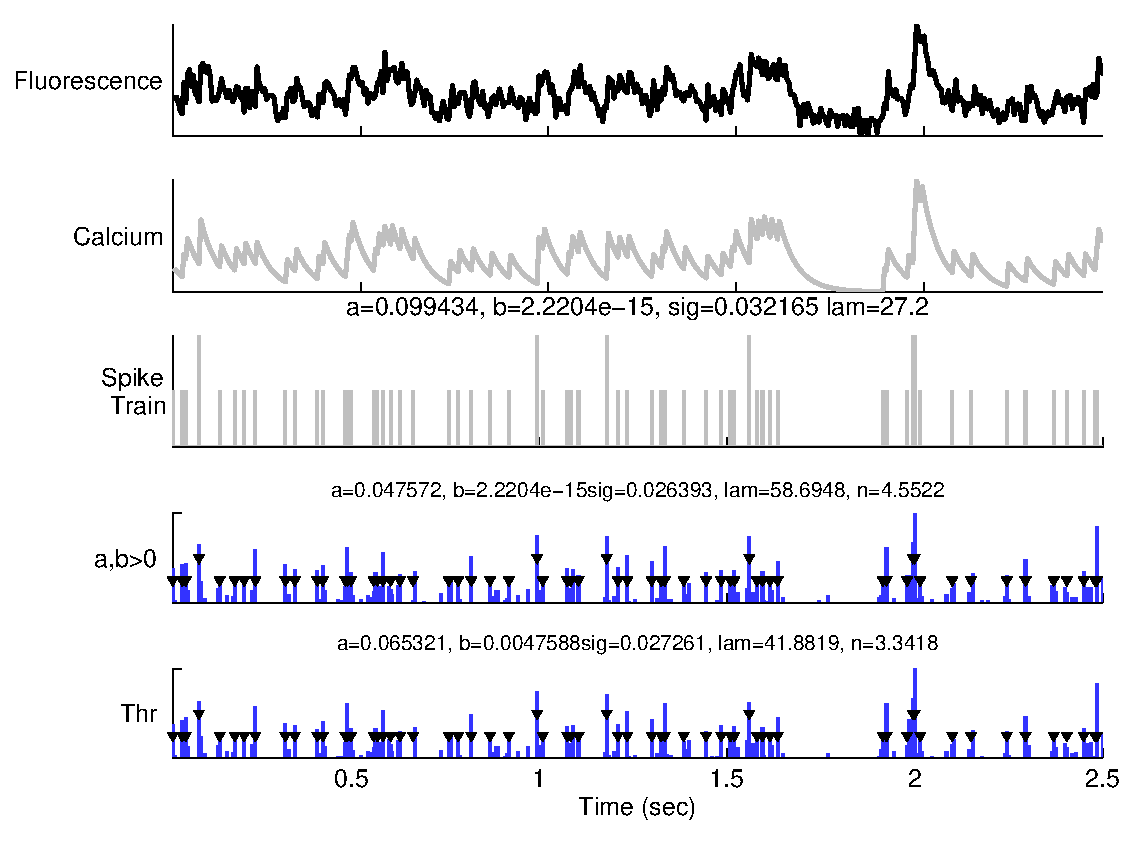
\includegraphics[width=.9\linewidth]{schem}
%\caption{full movie, fully automated} \label{fig:spatial_full}
%\end{figure}

\begin{figure}[h!]
%\centering 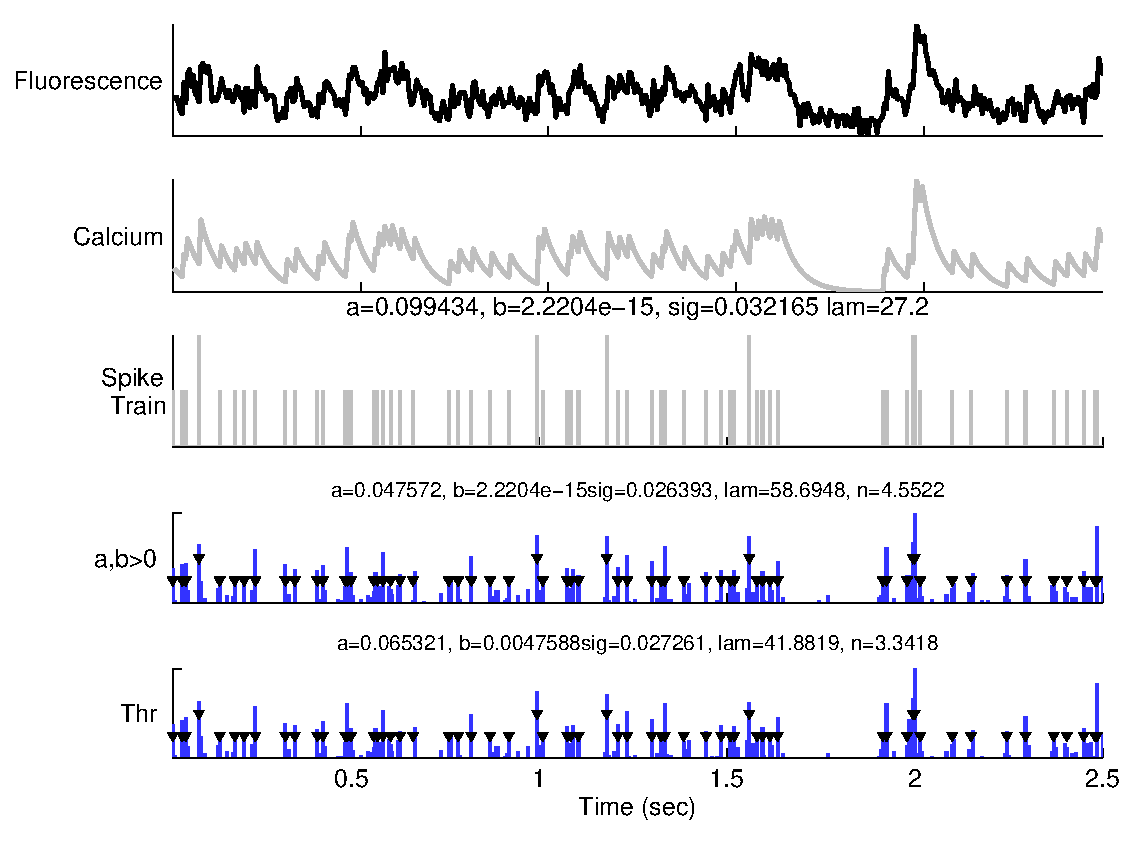
\includegraphics[width=.9\linewidth]{schem}
\caption{full movie, in vitro data} \label{fig:spatial_full_data}
\end{figure}



% 
% \clearpage\newpage
% \subsection{in vitro data} \label{sec:vitro}
% \input{tex/in_vitro}
% 
% \clearpage\newpage
% \subsection{in vivo data} \label{sec:vivo}
% 
\begin{figure}[H]
\centering 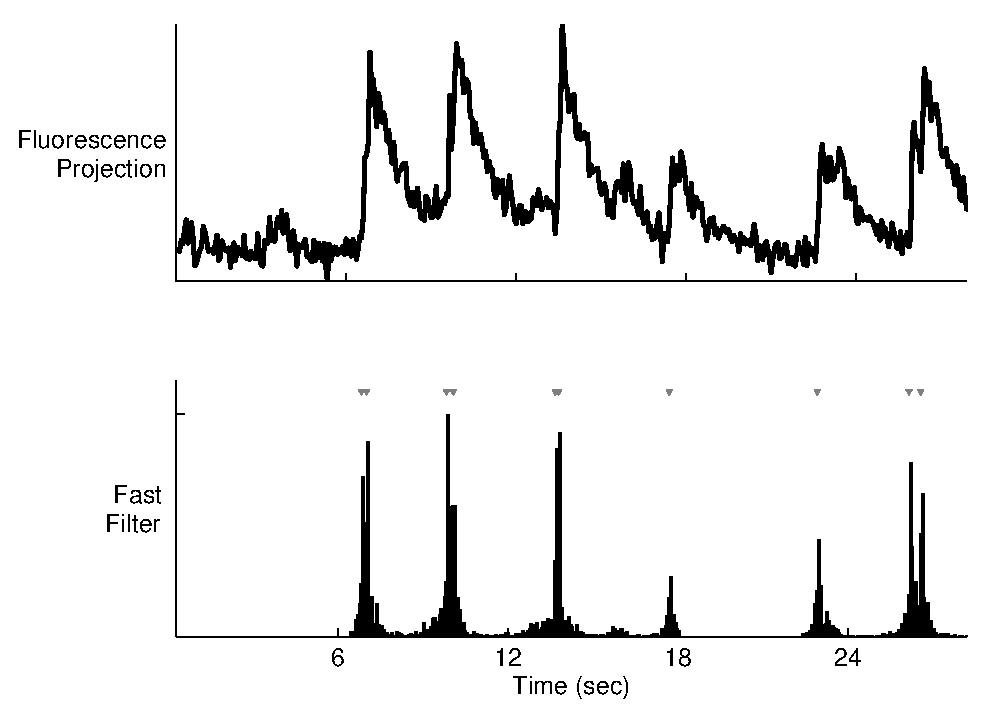
\includegraphics[width=.9\linewidth]{../figs/spatial_data}
\caption{Given only a fluorescence movie, recorded in vivo, we can learn the parameters necessary to correctly infer the spike trains. Top left: mean frame.  Middle left: projection of movie onto mean frame. Bottom left: the fast filter's inference using the mean frame as the filter ($\lam$ and $\sig$ estimated as described by equations \eqref{??} and \eqref{??}, respectively).  Right panels: same as left, but estimating $\balpha$ and $\bbeta$ as described in text.} \label{fig:spatial_data}
\end{figure}

\begin{figure}[H]
%\centering 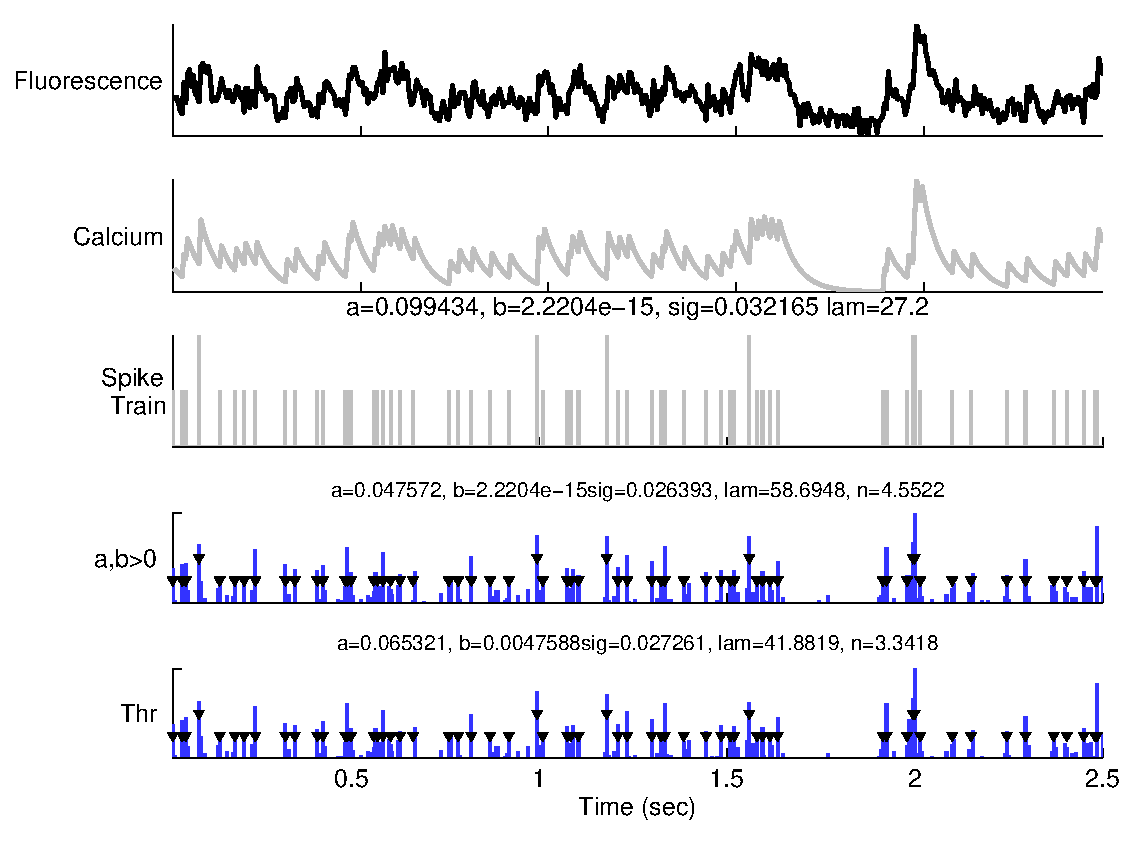
\includegraphics[width=.9\linewidth]{schem}
\caption{distribution of errors in spike inference from real data} \label{fig:err}
\end{figure}



% 
% \clearpage\newpage
% \subsection{Poisson observation model} \label{sec:poisson}
% \paragraph{Model}

\begin{align}
	\bF_{x,t} \sim \text{Poisson}(\alpha_x (C_t + \beta))
\end{align}

\paragraph{Inference}

\begin{subequations} 
\begin{align}
\mL_{x,t} &= -\alpha_x (C_t + \beta) + F_{x,t} \log(\alpha_x(C_t + \beta)) - \log(F_{x,t}!)  \\
g_{x,t} &= -\alpha_x + F_{x,t}(C_t + \beta)^{-1} \\
H_{x,t} &= -F_{x,t} (C_t + \beta)^{-2}
\end{align}
\end{subequations}

\noindent where $\mL=\sum_{x,t} \mL_{x,t}$, $\bg=\sum_x (g_{x,1}, \ldots, g_{x,T})\T$, and $\bH=\text{diag}(\sum_x H_{x,t})$.
% 
% \clearpage\newpage
% \subsection{Incorporating a nonlinear observation model} \label{sec:nonlin}
% \begin{align}
\bF_t &= \balpha S(C_t + \beta) +  \ve{\varepsilon}_t, \qquad &\ve{\varepsilon}_t \sim \mathcal{N}(\ve{0},\sig^2 \bI)
\end{align}

\noindent where $S(x)=\frac{x^{n_d}}{x^{n_d}+k_d}$

note: initialize with linear result, but add a constant wherever constraint is not satisfied
% 
% \clearpage\newpage
% \subsection{Slow rise time} \label{sec:slow}
% \begin{figure}[h!]
%\centering 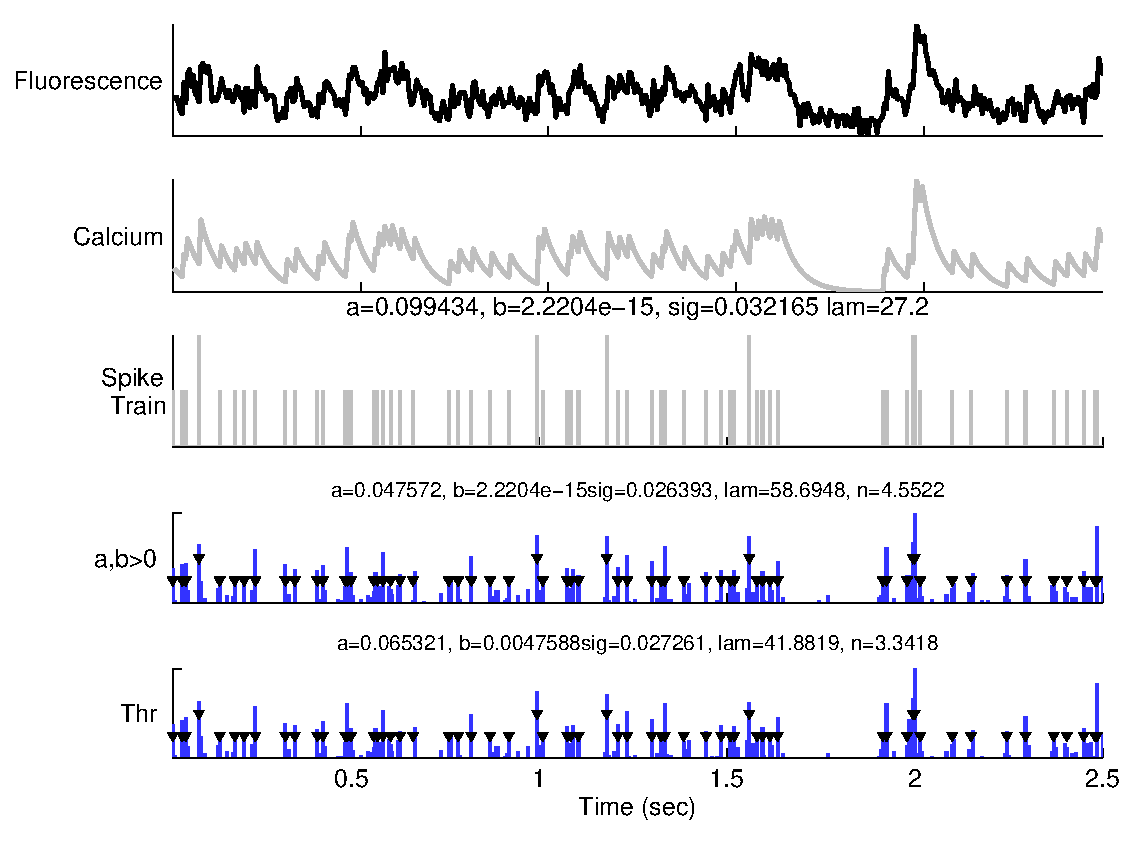
\includegraphics[width=.9\linewidth]{schem}
\caption{Slow rise time} \label{fig:slow}
\end{figure}



% 
% \clearpage\newpage
% \subsection{Dynamic prior}
% \paragraph{Model}

let $\blam = (\lam_1, \ldots, \lam_T)\T$

\begin{align}
	C_t &= \gam C_{t-1} + n_t, \qquad n_t \sim \text{Poisson}(n_t; \lam_t \Del)
\end{align}

\paragraph{Inference}

\begin{subequations} 
\begin{align}
\mL &=  \frac{1}{2 \sig^2} \norm{\bF - \balpha (\trans{\bC} +\beta+\ve{1}\T)}^2 + (\bM \bC )\T \blam \Del  - \zzz \log(\bM \bC)\T\ve{1} \\
\ve{g} &= -\frac{\balpha}{\sig^2}(\bF -\balpha({\hbC\T}_{\zzz} + \beta)) + \ve{M}\T \blam \Del  - \zzz \ve{M}\T (\ve{M} \hbC_{\zzz})^{-1}
\end{align}
\end{subequations}



\end{document}